%----------------------------------------------------------------------------------------
%	Trent Project Report Req's
%----------------------------------------------------------------------------------------

\documentclass[12pt,a4paper,oneside]{report}
\renewcommand{\baselinestretch}{1.5}
\usepackage[left=2.5cm,right=2.5cm,top=2.5cm,bottom=2.5cm]{geometry}

%----------------------------------------------------------------------------------------
%	Custom Packages
%----------------------------------------------------------------------------------------

\usepackage[utf8]{inputenc}
\usepackage{amsmath}
\usepackage{graphicx}
\usepackage[export]{adjustbox}
\usepackage{float}
\usepackage{url}
\usepackage{amsfonts}
\usepackage{amssymb}

\usepackage[titletoc, title]{appendix}
\usepackage{titlesec}
\usepackage{lipsum}
\usepackage{listings}
\usepackage{hyperref}
\hypersetup{%
    pdfborder = {0 0 0},
    colorlinks,
    citecolor=blue,
    filecolor=Darkgreen,
    linkcolor=red,
    urlcolor=blue
}

\usepackage{caption}
\captionsetup[figure]{labelfont={bf},labelformat={default},labelsep=period,name={Figure}}
\captionsetup[table]{labelfont={bf},labelformat={default},labelsep=period,name={Table}}

\usepackage{titling}
\newcommand{\subtitle}[1]{%
  \posttitle{%
    \par\end{center}
    \begin{center}\large#1\end{center}
    \vskip0.5em}%
}

\usepackage[table]{xcolor}

\usepackage[
  backend=bibtex
 ,style=numeric-comp 
 ,sorting=none   
 ,sortcites=true   
 ,block=none
 ,indexing=false
 ,citereset=none
 ,isbn=true
 ,url=true
 ,doi=true        
 ,natbib=true  
]{biblatex}
\addbibresource{Mendeley.bib} 


%----------------------------------------------------------------------------------------
%	Settings
%----------------------------------------------------------------------------------------

\begin{document}

\titleformat{\chapter}[display]
  {\normalfont\bfseries}{}{0pt}{\LARGE}

\lstset{language=Python,
    breaklines=true,
    morekeywords={matlab2tikz},
    keywordstyle=\color{blue},
    morekeywords=[2]{1}, keywordstyle=[2]{\color{black}},
    identifierstyle=\color{black},
    stringstyle=\color{red},
    commentstyle=\color{mygreen},
    showstringspaces=false,
    numbers=left,
    numberstyle={\tiny \color{black}},
    numbersep=9pt, 
}

\begin{titlepage}
\renewcommand{\baselinestretch}{1}
\centering
\vspace{5cm}
\textbf{\LARGE{Research into the feasibility of a new interferometer on MAST-U}} \\
\vspace{0.75cm}
\large{A literature review submitted in partial fulfilment of the requirements for MSci Physics \\} 
\vspace{1.5cm}
\textbf{\Large{Christopher James Hickling}} \\
\vspace{9cm} 

\begin{figure}[H]
\centering      

\includegraphics[width=10cm, height=10cm, keepaspectratio]{Images/ntulogo.jpg}
\end{figure}    

\large{School of Science and Technology} \\
\large{Nottingham Trent University} \\
\large{Clifton Lane} \\
\large{Nottingham} \\
\large{United Kingdom} \\
\vspace{1cm}
\large{2017}
\end{titlepage}


\tableofcontents
\pagebreak
\clearpage
\pagenumbering{arabic}

%----------------------------------------------------------------------------------------
%	Abstract
%----------------------------------------------------------------------------------------

%\chapter{Abstract}
%The aim of this project is to investigate and test the effectiveness of a new interferometer system for diagnostic purposes. This system is based on the use of a 1550nm laser diode \cite{KoheronLaserV1} interferometer system designed to measure the electron density of plasma in MAST-U (Mega Amp Spherical Tokamak - Upgrade).

%----------------------------------------------------------------------------------------
%	Introduction
%----------------------------------------------------------------------------------------
\chapter{Introduction}
Interferometry is a powerful diagnostic technique that is currently employed on nearly all experimental fusion reactors worldwide. In some cases the interferometer system is part of the real time diagnostics, and the reactor will not be allowed to function without it, for safety reasons. For the purposes of this literature review, the reactor MAST (Mega Amp Spherical TOKAMAK) will be used, as this is the reactor that the system will be implemented on.\\
The current interferometer system in place on MAST was designed by Jakob Brunner, as part of his PhD project \cite{Brunner2017}. The thesis brought up main concerns about the use of a CO$_{2}$ laser brings up many safety issues, that result in there only being potential for one interferometer to be used. This means that only a single line profile of density can be obtained within the reactor. This is not a good representation of the density fluctuations in the reactor, and also only passes through the bulk plasma.\\
The intention of this project is to replace the CO$_{2}$ laser with a 1550nm laser produced by Koheron \cite{KoheronLaserV1} along with Koheron's InGaAs photo detectors \cite{KoheronPD100Photodetector} as this will improve safety of the system which will allow multiple interferometers to be installed looking through various line of sights in MAST-U (MAST-Upgrade). Since this set-up also doesn't require a glass viewing port as the CO$_{2}$ laser does, this can allow for the interferometer to also pass through more interesting (density wise) points of the plasma, e.g. the divertor.

%----------------------------------------------------------------------------------------
%	Lit Review
%----------------------------------------------------------------------------------------

\chapter{Literature Review}
	\section{Nuclear Fusion}
Nuclear Fusion is the act by which two small nuclei are in close enough proximity and have the necessary energy to overcome the coulomb barrier and to fuse them together. This process releases vast amounts of NET energy and so has been a pedestal of scientific advancement since the mid 20th century. Fusion research became a field in the 1930's, reactors had very low collisionality and were large, with energy losses to match. It wouldn't be until 1957 that fusion was actually achieved in a laboratory setting with the ZETA reactor, then based at Culham Centre for Fusion Energy. Although this was a huge milestone for fusion research, it revealed that achieving fusion with a NET positive energy output was no easy task. Soon after the favoured reactor of choice called a Tokamak (loose transliteration of acronym: Toroidal Chamber with Magnetic Coils) came from a Russian group of scientists.
\\
Experiments up until this point had shown that plasma instabilities were common and ultimately a drain on a fusion's ability to self sustain its own reactions. This made fusion scientists realise that a large amount of data and diagnostics equipment is required to understand the physical principles at work inside the reactor.
\pagebreak
	\subsection{Underlying Physics}
The amount of energy released from a nuclear fusion reaction is dictated by the mass of the individual atoms before the reaction, and the products after the reaction. \linebreak

\begin{figure}[H]
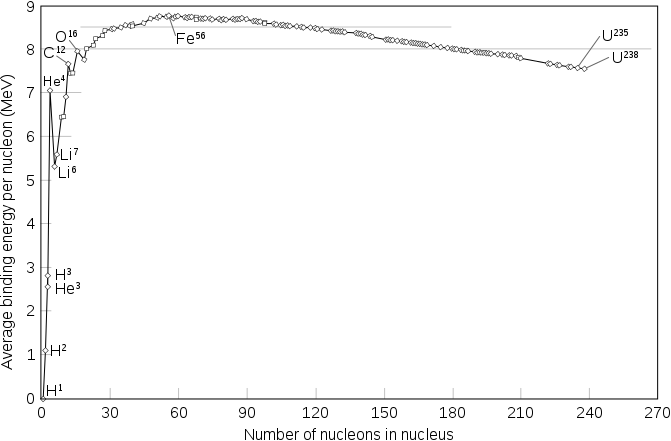
\includegraphics[width=0.9\textwidth, center]{Images/Bindingenergy.png}
\caption{The average binding energy of nucleons against the number of nucleons. This shows that a transition from one light element to another results in a large energy deficit, this is released as energy in a fusion reaction \cite{Fastfission2008BindingNucleon}}
\label{bindingenergy}
\end{figure}

As shown in \autoref{bindingenergy}, lighter elements have far less binding energy per nuclear than heavier elements. This means that, for example, combining two Hydrogen$^{1}$ atoms together will result in a Hydrogen$^{2}$ atom, plus an amount of energy that is released.

\begin{equation}
{^{1}H} + {^{1}H} = {^{2}_{1}H} + {^{1}_{0}e} + {\nu}^{-} + Energy
\end{equation}
\\
This process continues but with exponentially decreasing energy release up to iron. Iron is the heaviest element that can be achieved via fusion while still having a positive net energy output. The largest amount of energy from a single reaction can be achieved by fusing two atoms and gaining the largest mass deficit possible. The largest of these being a Deuterium-Tritium (D-T) reaction \cite[p. 430]{Shultis2016FundamentalsEdition.}:

\begin{equation}
{^{2}_{1}H} + {^{3}_{1}H} = {^{4}_{2}He} + {^{1}_{0}n} + 14.1MeV
\end{equation}

In this reaction, the neutron inherits the energy as kinetic energy. Very few reactors worldwide have attempted a D-T reaction, but those that have suffered significant damage from the high powered neutrons that have been released.

	\section{Tokamak}
Tokamak is an loosely translated acronym for a device developed by soviet Russia in the 1960's, it stands for \textbf{TO}roidal \textbf{CHA}mber with \textbf{MA}gnetic \textbf{C}oils. First results from such a machine were published in 1969 by two Russian scientists, Sakharov and Tamm \cite{Tamm1959TheoryI}. The Russian team managed to produce plasmas of a much higher stability than previously seen, and at temperatures up to 10 times higher than previously achieved. Since then, TOKAMAK development has been progressing, solving one problem at a time, but uncovering many new challenges in the fields of engineering, materials research and plasma physics \cite{Smirnov2010Tokamak19501990}.\\

In general, the longer that a fusion plasma can be confined (under fusion conditions), the more probability of fusion reactions taking place. There are two main ways to increase confinement time; an increase of radius of a reactor or an increase in magnetic pressure. Magnets are currently approaching the limit of what we can achieve with superconducting technology, so the favoured solution is to increase the size of the reactor. For the purposes of analysing plasma phenomena and performing research a reactor just the right size to fit on all the diagnostics required is adequate, which is the reason behind the building of MAST \cite{Chapman2015OverviewResults}\\

MAST is currently in the process of being upgraded into MAST-U, where is will have many improved features including a new divertor region that allows for more complex plasma configurations and longer path length, which allows the plasma to slow down (and cool down) before striking the divertor plate (\autoref{mastdivertors}, \cite{CulhamCenterforFusionEnergyResearch:Upgrade})

\begin{figure}[H]
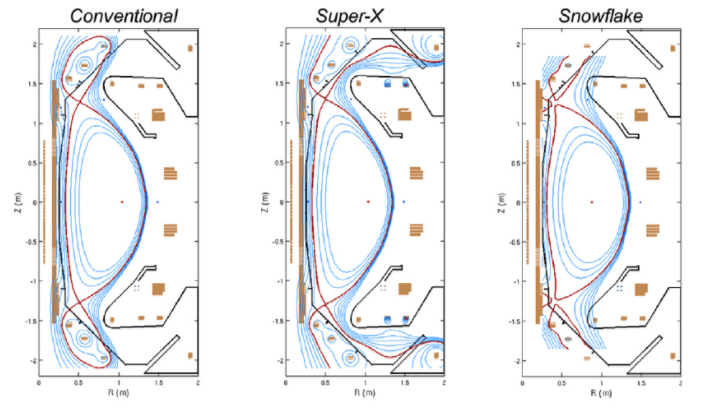
\includegraphics[width=1\textwidth, center,angle=0]{Images/MASTUdivertors}
\caption{MAST-U divertor regions derived by free vacuum boundary calculations. Shows 3 possible new configurations of the magnetic field and ion path passing through the divertor \cite{CulhamCenterforFusionEnergyResearch:Upgrade}.}
\label{mastdivertors}
\end{figure}

	\section{Diagnostics}
There are many forms of diagnostics in a fusion reactor. These can be separated into two different groups; Real Time Diagnostics and Delayed Diagnostics. Real Time Diagnostics collect data, analyse it and feed it straight back into the system. They are used to make quick changes to try and harness instabilities or to cause a shut down if something goes wrong. Delayed Diagnostics aim to just collect data of a pulse in order for scientists to analyse it at a later time. This is useful for building an understanding of the physical process without sacrificing processing time to analysing data, only collecting it. 
\medskip

One of the main challenges of fusion research, currently, is to limit instabilities generated by Edge Localised Modes (ELMs). This is a disruptive instability that occurs in the edge of a reactor plasma. These instabilities can seriously damage the reactor wall (particularly divertor plates) as well as causing massive energy losses of the plasma. Ultimately instabilities such as this limit the time that a fusion reactor can run for.
	
	\section{Basic Interferometry}
Interferometry is a method by which time-integrated plasma density can be obtained. An interferometer, by design, is an incredibly sensitive piece of measuring apparatus. They work on the principle of interference between two laser beam paths. If a laser is split into two beam paths of uneven lengths, an interference pattern will form if they are recombined. The rate at which this interference pattern "chirps" (A creation or destruction of a waveform takes place) is proportional to the difference in path length of the arms. If, for example, the path lengths were identical, no interference would take place upon recombination. By inserting a plasma into one of these arms a path difference will become apparent. This path difference is proportional to the line-integrated density of the plasma. This is due to the density-dependant refractive index of the plasma. A larger density results in a larger refractive index, and hence the laser has an apparent path of greater length than before.

In a plasma the optical path in a double pass interferometer (passing through the plasma twice) can be calculated according to the following equation \cite[p.~26]{Brunner2017} :

\begin{equation}
	\Delta s = 2 \int_{0}^{L} [N_{air} - N_{pl}(l)]dl \approx 2 \int_{0}^{L} \Bigg[1 - \sqrt[]{1-\frac{\omega_{pe}^{2}}{\omega^{2}}}\Bigg]
	\label{opticalpathint}
\end{equation}

Where $N_{pl}$ denotes the plasma's refractive index that already includes the visible light approximation. $N_{air}$ is the refractive index of air. $\omega$ is the frequency of the laser and $\omega_{pe}$ is the frequency of the plasma. This can then be expanded by assuming that the plasma frequency is much less than the frequency of the laser to achieve:

\begin{equation}
	\Delta\phi_{pl} \approx \frac{\lambda e^{2}}{2 \pi c^{2} \epsilon_{0} m_{e}} \int_{0}^{L} n_{pl} (l) dl
	\label{phase}
\end{equation}

\begin{equation}
	\int_{0}^{L} n_{pl} (l) dl = \frac{2 \pi c^{2} \epsilon_{0} m_{e}}{\lambda e^{2}} \Delta\phi_{pl} = \frac{\lambda n_{c}}{2 \pi} \Delta\phi_{pl}
	\label{phaseintegral}
\end{equation}
\\
Where $\Delta\phi_{pl}$ is the phase difference between the two interferometer arms. $\lambda$ is the wavelength of the laser used. e and c are the electron charge and the speed of light in a vacuum, respectively. $\epsilon$ permittivity of free space and $m_{e}$ is the mass of the electron. $n{pl}$ is the density of the plasma, which in an ideal hydrogen plasma can be defined entirely by the density of the electrons as the Debye length of the ions is on too large a scale for the measurement to make a contribution. 

This now gives a viable way to calculate the change in phase of a laser passing through plasma. Providing the precise distance of the beam path within the reactor is known with a precision to the order of the wavelength of the laser. Unfortunately the vibration of the machine causes this value to fluctuate causing uncertainty in the phase. For this reason two different colour lasers that follow the same beam path must be implemented. One must interact strongly with the plasma and the wall, the other must interact weakly with the plasma and strongly with the wall.


\begin{figure}[H]
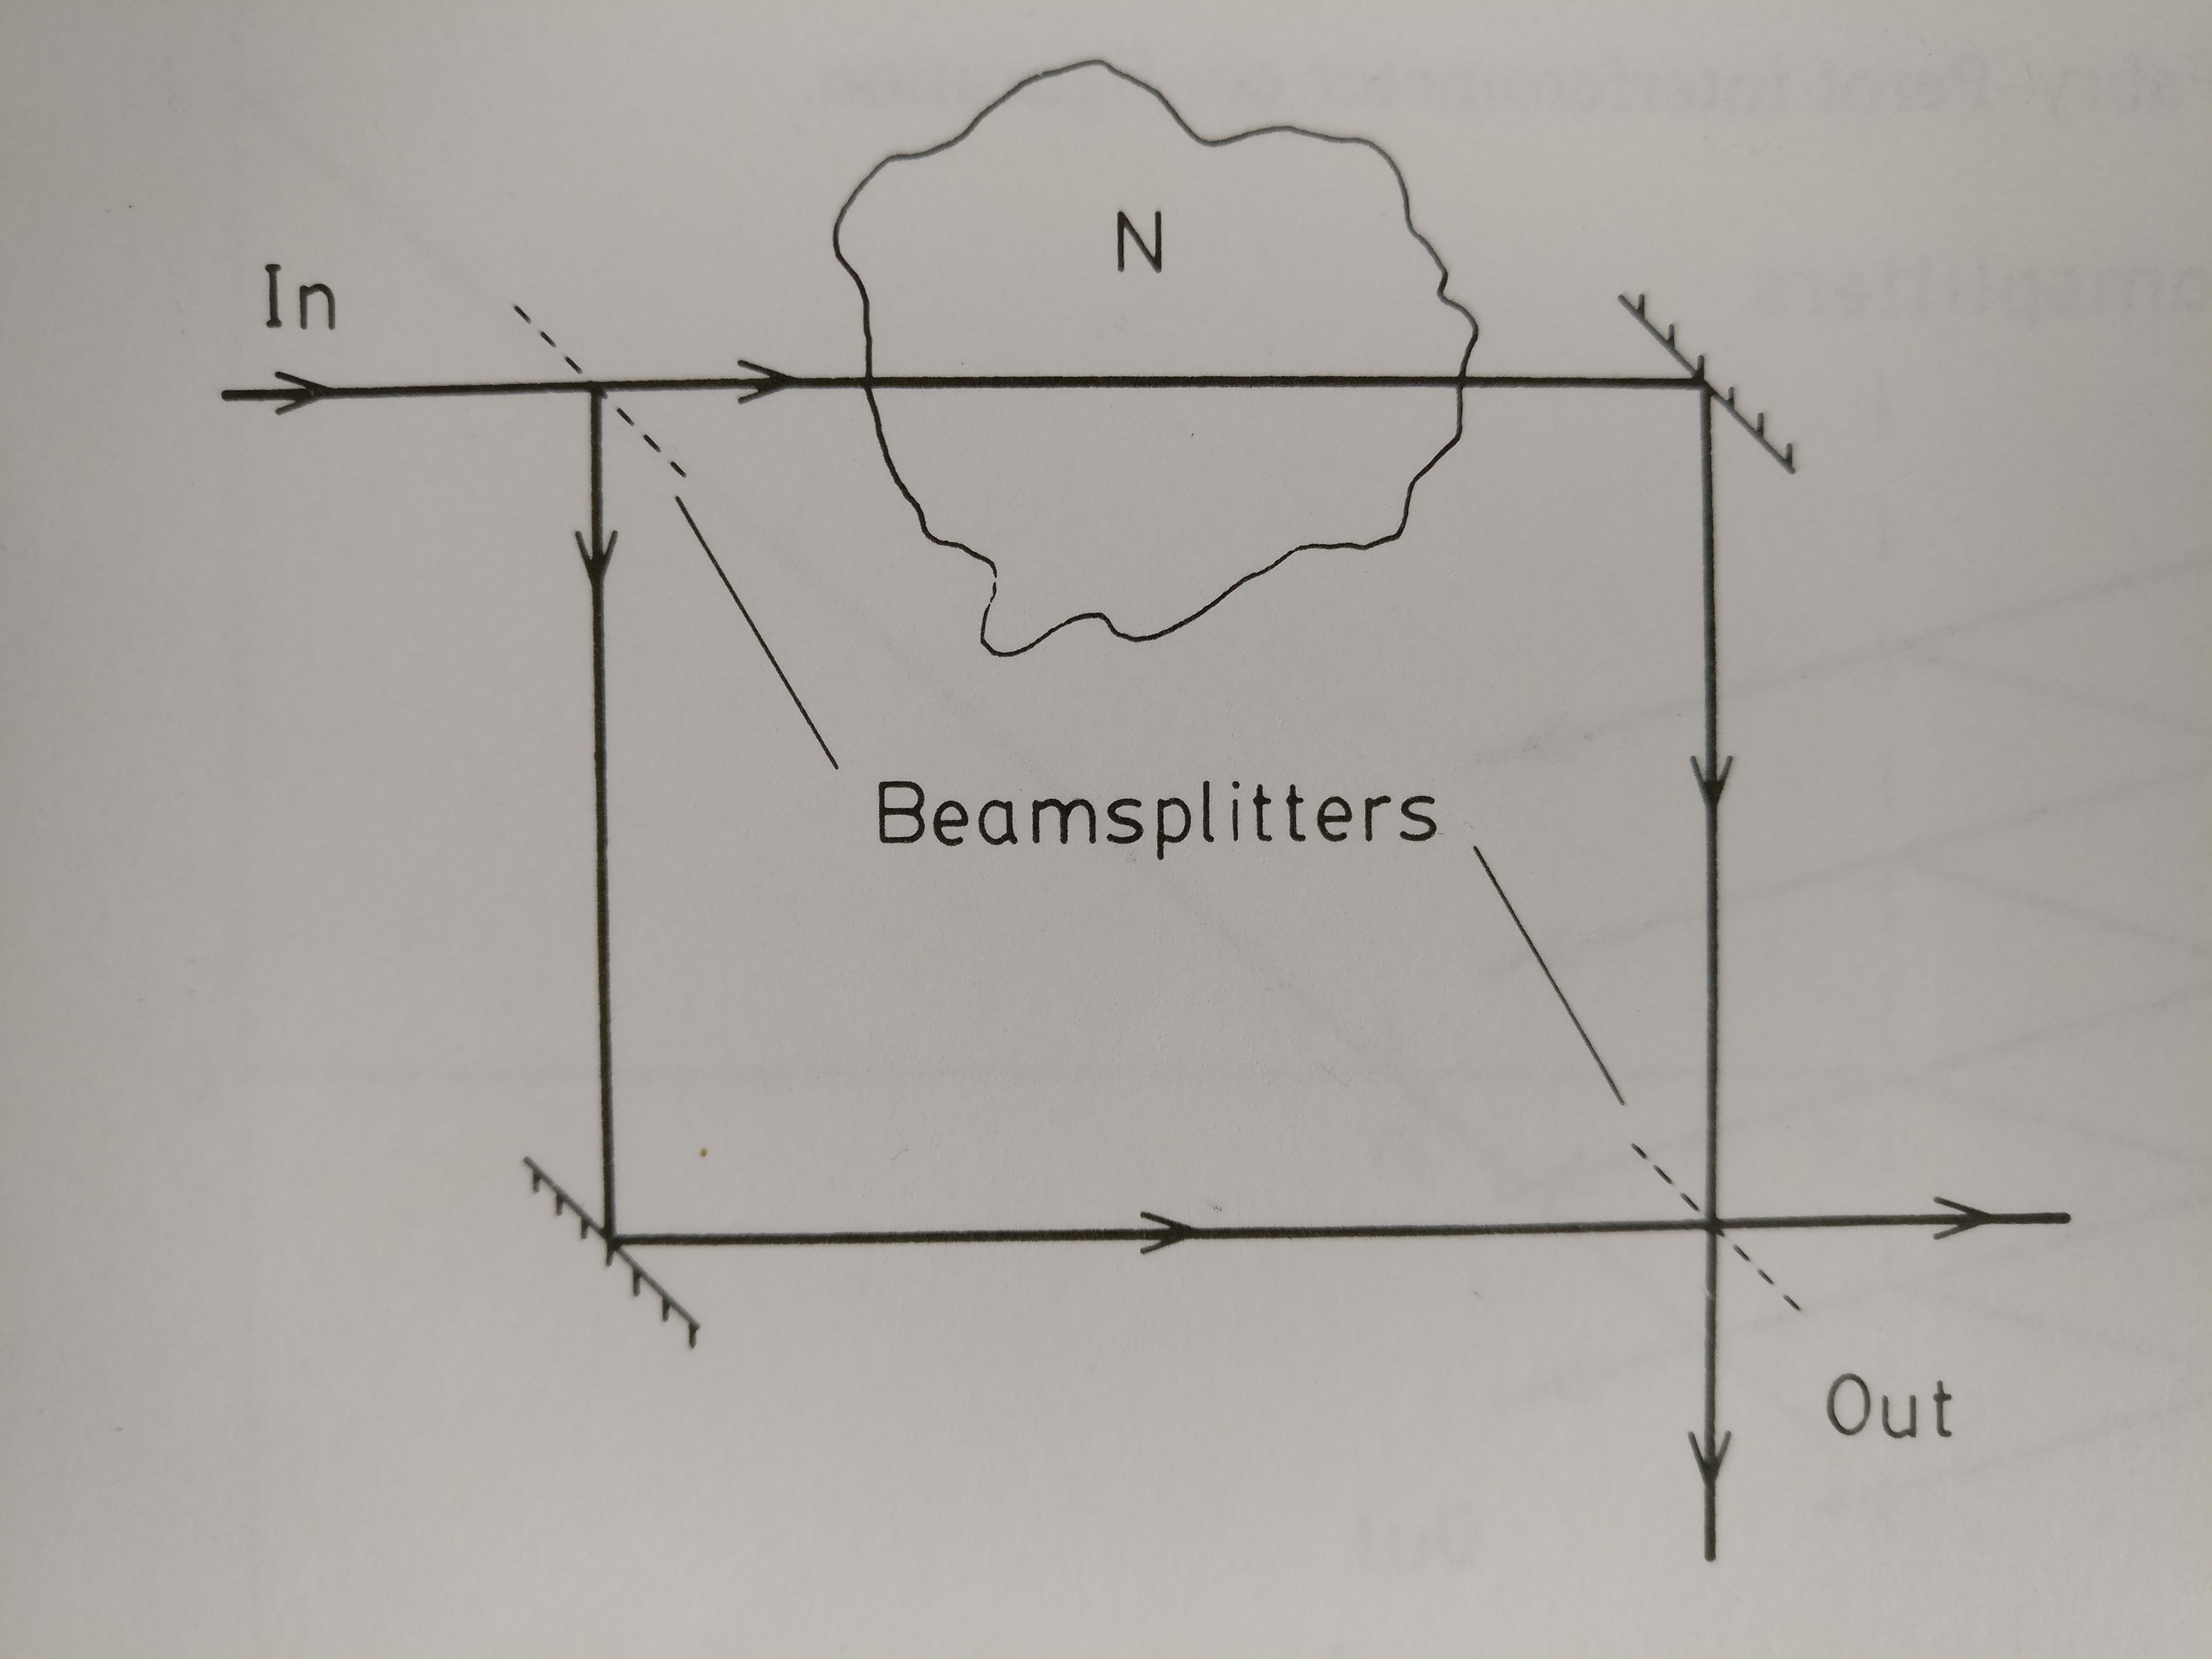
\includegraphics[width=0.6\textwidth, center,angle=0]{Images/mzint.jpg}
\caption{A schematic for a Mach-Zehnder interferometer where the Region N corresponds to a region of plasma. Image taken from Principles of Plasma Diagnostics \cite[p.~97]{Hutchinson2005PrinciplesDiagnostics}}
\label{mzint}
\end{figure}

	\subsection{Heterodyne Interferometry}
A heterodyne (two colour) interferometer is a system that applies two different wavelength light sources into a single interferometer system. When the light interferes a beat frequency is produced which can be used to compute the phase difference between the two light sources. This is done with little dependence on the signal amplitude, and so the strength of the signal is of little relevance so long as the wavelengths are unique and can be distinguished from a background. In addition to the physical benefits, this optical set up can also be applied to negate certain engineering effects created by the system. One issue which was found in early research is that fusion reactors actually vibrate with a specific frequency and in some cases can shift several millimetres relative to the beam path. This means that the effect of this vibration cant be differentiated from a change in density of the plasma. One way that has been found to counter this is two employ a two colour system where one laser has strong interaction with the plasma, and the other laser has weak or little interaction with it, these are usually a mid-infrared (e.g. CO$_{2}$) and a visible (HeNe). This results in the visible laser having a phase change relative to the vibration of the reactor, and the mid-infrared has phase changes resulting from the plasma and the reactor. If these two laser systems follow identical beam paths and are calibrated correctly, the phase of the visible can be subtracted from the phase of the mid-infrared resulting in the phase change caused by the plasma alone.\\

	\section{Measuring Displacement using Heterodyne Interferometry}
By comparing the signal between two different detectors that are suited for each wavelength of the heterodyne system information can be extracted regarding the difference in phase. This will result in a time-varying signal on both the scene and the reference arm of the interferometer which can be calculated using a series of equations in the form of \cite{WuHeterodyneNanometrology}

\begin{equation}
	I{_{s}} \propto A{_{s}}\cos{(\Delta\omega t + \phi{t})}
    \label{SceneInt}
\end{equation}
and
\begin{equation}
	I{_{r}} \propto A{_{r}}\cos{(\Delta\omega t)}
    \label{RefInt}
\end{equation}
Where $A{_{s}}$ and $A{_{r}}$ are the amplitudes of the scene and reference arms respectively, $\omega$ is the angular frequency of the signal and $\phi$ is the phase.


    
    
The general equation to extract the plasma density from a heterodyne system \cite{Esteban2010ContinuousFPGAs} is given by \autoref{eq:density}. A full derivation can be found in Jakob Brunner's Thesis \cite[p. 22-29]{Brunner2017}

\begin{equation}
	\int{n_{e}dl} = n_{e}(CO_{2})\frac{\Delta\psi_{NdYAG}\lambda_{NdYAG}-\Delta\psi_{CO_{2}}\lambda_{CO_{2}}}{2\pi}
    \label{eq:density}
\end{equation}
\begin{figure}[H]
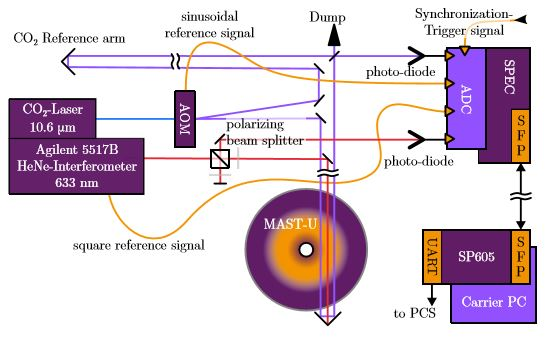
\includegraphics[width=\textwidth, center,angle=0]{Images/mastuint.JPG}
\label{MAST-U Int}
\caption{A schematic of the interferometer currently in place on MAST-U. This shows the complexity of the system and the difficulty of expanding it to include more interferometers. \cite{Brunner2017}}
\end{figure}

Currently in MAST (Mega Amp Spherical Tokamak) a heterodyne system is in place. This consists of a $CO_{2}$ laser in combination with a HeNe laser integrated with a FPGA system designed by J.K.Brunner \cite{Brunner2017}. So long as the modulation frequency of each of the lasers is known to a high precision, the plasma density can then be derived by a calculation of relative phase between the two lasers. One of the largest limitations to this system is the temperature dependence of the CO2 laser. The laser needs to be cooled otherwise it will have slight fluctuations in its output which will affect the phase calculation.\\
Another limitation is the cost of the $CO_{2}$ laser, as it is very expensive and requires a large amount of maintenance. The wavelength of the laser is chosen to have strong interaction with the plasma, but unfortunately it also has strong interaction with human skin and eyes. As a result this laser has very strict safety precautions and requirements that come with its installation. These precautions are made more apparent since the laser has to enter the vacuum vessel via a glass viewing port which leaves the beam path exposed for a short distance.

	\section{Field Programmable Gate Array's (FPGA's)}
FPGA's are a simple and effective way to collect and analyse data. They have numerous advantages over standard processing devices as they are designed to compute a single pre-programmed task, as unlike a Central Processing Unit (CPU) which is designed to use logic to solve a specific task. The use of an FPGA is becoming more common in fusion applications as the need to perform real time filtering \cite{Naylor2010AnMAST} and processing on data is becoming a greater concern for plasma control systems to allow the safe operation of reactors. Many different forms of FPGA's have been used in the fusion industry for real time application.
	\subsection{Red Pitaya}
    
The Red Pitaya (RP) \cite{Leban2014RedManual} is a micro controller that has built in FPGA capabilities. This is further simplified by Koheron by designing software for the RP to run, which includes an oscilloscope and spectrum analysis software as well as control of the laser's modulation frequency and current, through a simple interface.

%The Red Pitaya (RP) \cite{Leban2014RedManual} is a open source micro controller with a built in Field Programmable Gate Array (FPGA) with a very user friendly user interface. It operates two inputs and two outputs at 125MS/s. FPGA's are notorious for being difficult to program as they are intrinsically complicated. The stand out function of a FPGA is the way it processes information. It can perform many tasks in parallel pipelined processing i.e. performing the same operation on many data sets. The number of parallel pipelines that can be implemented depends entirely on the hardware limitations of the FPGA. This often means that the limiting factor of the speed at which a RP can process data is the speed at which you can transmit data to it. This gives FPGA's a large advantage over conventional computers when it comes to real time data applications.

\begin{figure}[H]
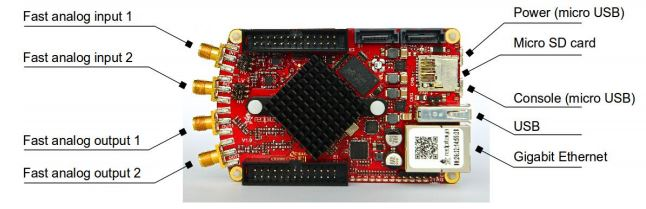
\includegraphics[width=0.9\textwidth, center,angle=0]{Images/RP.JPG}
\caption{The Red Pitaya showing all the connected ports. Each of the analogue ports can sample at 125MHz \cite[p.~7]{Leban2014RedManual}.}
\label{RP}
\end{figure}

\begin{table}[H]
	\setlength\arrayrulewidth{1pt}
    \rowcolors{2}{gray!25}{white}
    \begin{tabular}{ c c c c } 
        Name & Type & Connector & Description\\
        \hline
        IN1/IN2 & Input & SMA-F & RF input(High-Z, 1M$\Omega$ // 10pF\\[1pt]
        OUT1 / OUT2 & Output & SMA-F & RF output (50$\Omega$)\\[1pt]
        Ethernet & Full Duplex & RJ45 & 1000 Base-T Ethernet Connection\\[1pt]
        USB & Full Duplex & A USB & Used for standard USB Devices\\[1pt]
        Micro USB (Console) & Full Duplex & Micro B USB & Used for console connection\\[1pt]
        Micro USB (Power) & Input & Micro B USB & 5V / 2A power supply\\[1pt]
        Micro SD & Full Duplex & Micro SD slot & Micro SD memory card\\
    \end{tabular}
    \caption{Full Specifications of the Red Pitaya's input/output ports. Both fast analogue inputs and fast analogue outputs operate at 125MHz per channel \cite[p.~7]{Leban2014RedManual}.}
    \label{RPspec}
\end{table}

\section{Koheron}
Initial investigations at CCFE \cite{Hickling2017InvestigationMAST-U} have shown this method to show a strong interference pattern and the use of the RP and Koheron software is easy and accessible. There is a large amount of support and development occurring constantly so any new problems found can be fixed. In this investigation it was shown that the basic interferometer setup from Koheron is not currently sensitive enough to physical vibrations on the order of 10's of KHz. It was found that this may be due to the lack of any high order modulation of the laser due to an Acousto-Optical Modulator, as discussed by J. Brunner \cite[p. ~29]{Brunner2017}.

\pagebreak
\chapter{Bibliography}
	\printbibliography[heading=none]

\pagebreak

%----------------------------------------------------------------------------------------
%	Appendix
%----------------------------------------------------------------------------------------

\pagenumbering{roman}
\setcounter{page}{2}
\begin{appendices}

%\includepdf[pages={ - }]{ChristopherHicklingSummerProject.pdf}
\end{appendices}

\end{document}